
\subsubsection{GameManager} Principale elemento relativo al controller ed ha varie funzionalità, una di queste è \textit{initializeGame}, per l'inizializzazione del gioco: questo metodo permette di inizializzare la parte di \textit{GameView}, inoltre permette il caricamento di tutte le sprites utilizzate successivamente nella partita.
    \textit{GameManager} rappresenta un ponte tra la \textit{GameView} e \textit{GameLogic}, in quanto ascolta gli eventi compiuti dall'utente lato \textit{GameView} e li comunica al \textit{GameLogic}. 
    Per osservare gli eventi della view il \textit{GameManager} implementa il \textit{ViewObserver}, che verrà approfondito in un'altra sezione.
    inoltre il \textit{GameManager} implementa il \textit{GameLogicObserver}, si è scelto di usare il pattern observer per permettere al \textit{GameLogic} di notificare ogni qual volta viene eseguita un azione. Questo viene poi sfruttato dal GameManager per la riproduzione dei suoni.
    
    \subsubsection{GameLoop} Si è scelto di utilizzare un approccio ad event-loop single-thread per gestire le dinamiche di gioco. In accordo con i colleghi, questo approccio è stato scelto poichè si adatta bene al tipo di gioco sviluppato: il \textit{GameLoop} ha in particolare due task fondamentali da svolgere in sequenza, ovvero deve aggiornare la parte di \textit{GameLogic} e successivamente aggiornare la parte di \textit{GameView}. Inoltre l'approccio a event-loop, essendo in esecuzione su un singolo thread e processando un task alla volta, risulta essere thread safe.
    Quindi questa classe è incaricata di implementare l'Event-loop: all'avvio della partita il \textit{GameManager} fa partire un thread separato sul quale viene lanciato un event-loop incaricato di aggiornare la parte view ed, ad ogni ciclo, far compiere uno step alla parte logica.
    Per gestire gli eventi generati dall'utente vengono utilizzate due queue che tengono traccia degli spari e dei movimenti compiuti dall'utente e non ancora processati dall'event-loop. Gli eventi vengono poi recuperati ad ogni step come riportato in figura \ref{checknewMovement}, e passati al \textit{GameState} che li elaborerà. 
    
    \begin{figure}[H]
    \centering
      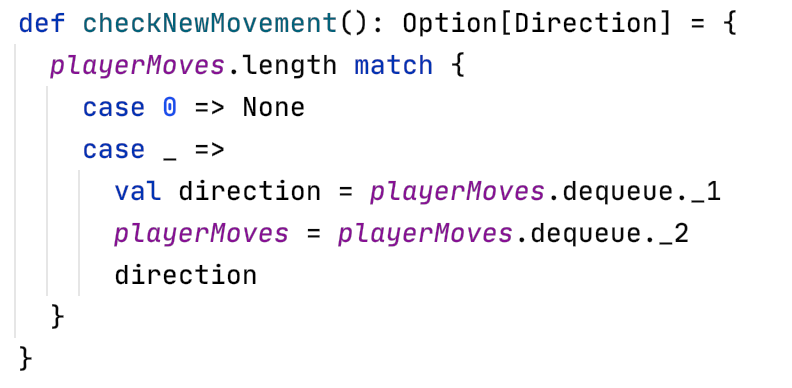
\includegraphics[width=10cm]{res/checkNewMovement.png}
      \caption{Recupera un movimento notificato}
      \label{checknewMovement}
    \end{figure}
    
    Una struttura generale della gestione degli eventi è riportata in figura \ref{gameLoop}: \textit{FXGameScene} rappresenta l'emitter degli eventi, che vengono poi, tramite \textit{GameManager}, salvati in due queue da cui il \textit{GameLoop} recupererà i singoli eventi e li darà in pasto al \textit{GameState}.
    
    \begin{figure}[H]
    \centering
      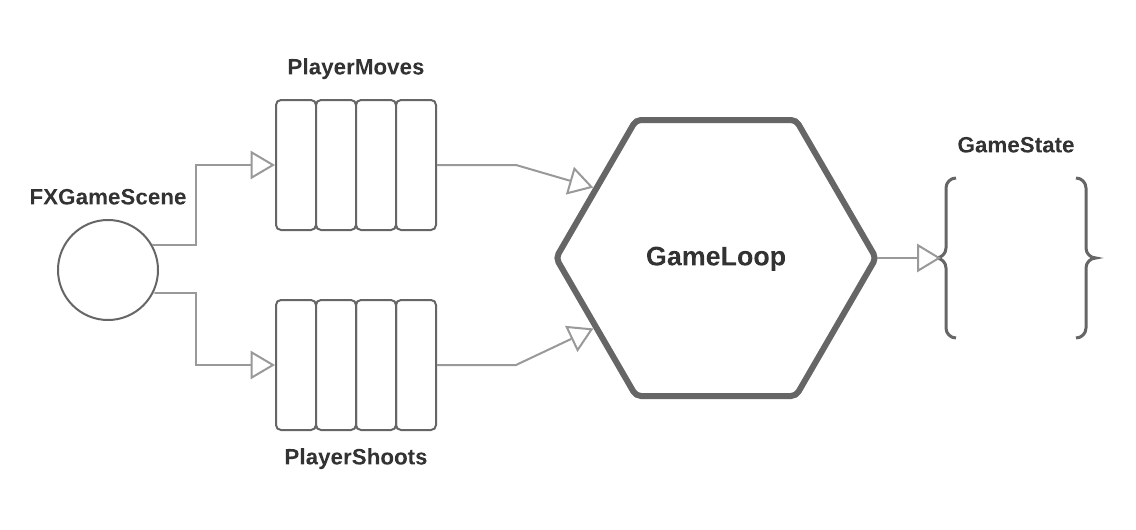
\includegraphics[width=14cm]{res/event_loop_diagram.png}
      \caption{Struttura gestione eventi}
      \label{gameLoop}
    \end{figure}
    
    \subsubsection{ImageLoader} Come accennato in precedenza, esso permette, all'apertura dell'applicazione, di caricare tutte le sprites utilizzate successivamente, in modo da limitare le letture da file durante l'esecuzione del gioco; questa operazione è fatta sfruttanto il meccanismo delle Future, quindi al suo completamento verrà visualizzata la finestra dell'applicazione. 
    Durante l'esecuzione del gioco invece permette alla \textit{GameView} di recuperare le \textit{Image} di cui ha bisogno.
    
    \subsubsection{SoundLoader} Gestisce la riproduzione dei suoni all'interno del gioco. Quando viene richiesta la riproduzione di un suono, viene generata una nuova \textit{Future} che creerà lo stream e quindi il clip per poi riprodurlo.
